Un agriculteur produit des bottes de pailles parallélépipédiques.

\begin{description}
\item[Information \textcolor{red}{1}] Dimensions des bottes de paille: 90~cm$\times$45~cm$\times$35~cm.
\begin{center}
\begin{tikzpicture}
\tkzDefPoints{0/0/A,2/-1/B,2.5/-.5/C,0/1.3/F,2.5/.8/D,.5/.5/G,.5/1.8/E,2/.3/H}
\tkzDrawSegments(A,B B,C C,D D,E E,F F,A F,H B,H H,D)
\tkzDrawSegments[dashed](E,G A,G G,C)
\end{tikzpicture}
\end{center}
\item[Information \textcolor{blue}{2}] Le prix de la paille est de 40~\eurologo{} par tonne.
\item[Information \textcolor{green}{3}] 1~m$^3$ de paille a une masse de 90~Kg.
\end{description}
\begin{enumerate}
\item Prix d'une botte de paille:
\begin{description}
\item[\textcolor{red}{1}] Volume: $V_{\text{botte}}=90\times 45\times 35=\nombre{141750}~\text{cm}^3=\nombre{0,14175}~\text{m}^3$
\item[\textcolor{green}{3}] Masse: $m_{\text{botte}}=\nombre{0,14175}\times 90=\nombre{12,7575}~\text{Kg}=\nombre{0,0127575}~\text{t}$ 
\item[\textcolor{blue}{2}] Prix: $P_{\text{botte}}=\nombre{0,0127575}\times 40\simeq 0,51$~\eurologo{} arrondi au centime.
\end{description}
\item Marc veut refaire l'isolation de la toiture d'un bâtiment avec des bottes de pailles parallélépipédiques. Le bâtiment est un prisme droit dont les dimensions sont données sur le schéma ci-dessous.

Il disposera les bottes de paille sur la surface correspondant à la zone grisée, pour créer une isolation de 35~cm d'épaisseur. Pour calculer le nombre de bottes de pailles qu'il doit commander, il considère que les bottes sont disposées les unes contre les autres. Il ne tient pas compte de l'épaisseur des planches entre lesquelles il insère les bottes.
\begin{enumerate}
\item Nombre de bottes nécessaires:
\begin{itemize}
\item Largeur du toit: C'est un rectangle, nous devons donc connaître la longueur: 15,3~m et la largeur $JF$: 
\[
JF^2=JI^2+IF^2=(7,7-5)^2+3,6^2=20,25\Longrightarrow JF=\sqrt{20,25}=4,5~\text{m}
\]
\item Nombre de bottes: comme l'indique la photo, il dispose les bottes dans le sens $J\to F$; il peut donc mettre $4,5\div 0,9=5$ bottes dans la largeur et $15,3\div 0,45=34$ bottes dans la longueur.
\end{itemize}
Il doit donc acheter $5\times 34=170$ bottes pour couvrir son toit.
\begin{center}
\begin{tikzpicture}
\tkzDefPoints{0/0/A,2/0/B,0/3/I,0/4.5/J,2/3/F,5/1/C,5/4/G,3/5.5/K,.4/4.2/B1}%
\tkzDefPointBy[homothety=center J ratio .1](K) \tkzGetPoint{B'2}
\tkzDefPointBy[translation=from J to B'2](B1) \tkzGetPoint{B2}
\tkzDrawPolygon[fill=gray](J,F,G,K) \tkzDrawPolygon(A,B,F,J)
\tkzDrawPolygon(B,C,G,F) \tkzDrawPolygon[fill=yellow](B1,B2,B'2,J)) 
\tkzDrawSegment(F,I)
\draw [<->,>=latex] (-.3,0)--(-.3,4.5) node[midway,sloped,fill=white]{7,7~m};
\draw [<->,>=latex] (0,-.3)--(2,-.3) node[midway,sloped,fill=white]{3,6~m};
\draw [<->,>=latex] (5.1,.7)--(2.1,-.3) node[midway,sloped,fill=white]{15,3~m};
\draw [<->,>=latex] (5.3,1)--(5.3,4) node[midway,sloped,fill=white]{5~m};
\tkzMarkRightAngle(F,I,J)
\tkzLabelPoint[above right](A){$A$} \tkzLabelPoint[above left](B){$B$} 
\tkzLabelPoint[below right](C){$C$} \tkzLabelPoint[above](K){$K$} 
\tkzLabelPoint[above right](G){$G$} \tkzLabelPoint[above](J){$J$} 
\tkzLabelPoint[below right](I){$I$} \tkzLabelPoint[below right](F){$F$} 
\end{tikzpicture}\hfill
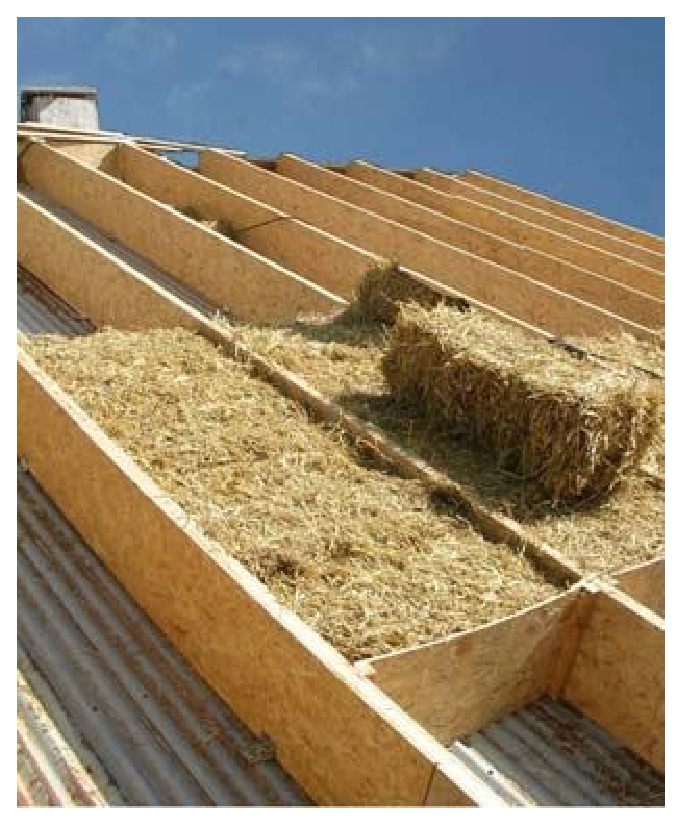
\includegraphics[width=.25\textwidth]{images-004.eps} 
\end{center}
\item Le coût de la paille nécessaire pour isoler le toit:
\[
170\times 0,51=86,70\ (\text{\eurologo})
\]
\end{enumerate}
\end{enumerate}

